\documentclass[11pt,spanish]{article}
\usepackage[utf8]{inputenc}
\usepackage{babel}
\usepackage{fullpage}
\usepackage{listings}
\usepackage{mathpazo}
\usepackage{enumitem}
\usepackage{courier}
\usepackage{xcolor}
\usepackage{textcomp}
\usepackage{amsmath}
\usepackage{amssymb}
\usepackage{tikz}
\usepackage{fancyhdr}
\usepackage{graphics}
\usepackage{array}

\newcommand{\titulo}{Certamen 1 [SJ, v1], miércoles 19 de diciembre de 2011}
\newcommand{\cc}[1]{\hfil\texttt{#1}\hfil}
\newcommand{\pond}[1]{[{\small\textbf{#1\%}}]}

\pagestyle{fancy}
\lhead{%
  {\Large\bfseries Programación---\titulo} \\
  Nombre: \nombre\hfill
  Rol:    \rol
  \vspace{2ex}
}
\chead{}\rhead{}\lfoot{}\cfoot{}\rfoot{}
\renewcommand{\headrulewidth}{0pt}
\addtolength{\headheight}{7ex}
\headsep=4ex


\newcommand{\onelinerule}{\rule[2.3ex]{0pt}{0pt}}
\newcommand{\twolinerule}{\rule[6.2ex]{0pt}{0pt}}
\newcommand{\respuesta}{\framebox[\textwidth]{\twolinerule}}
\newcommand{\nombre}{%
  \begin{tikzpicture}[xscale=.4,yscale=.7]
    \draw (0, 0) rectangle (22, 1);
  \end{tikzpicture}%
}
%\newcommand{\rol}   {\framebox[0.3\textwidth]{\onelinerule}}
\newcommand{\rol}{%
  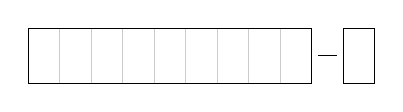
\begin{tikzpicture}[xscale=.4,yscale=.7]
    \draw[gray!40] ( 0, 0) grid      ( 9, 1);
    \draw          ( 0, 0) rectangle ( 9, 1);
    \draw          (10, 0) rectangle (11, 1);
    \draw (9 + .2, .5) -- (10 - .2, .5);
  \end{tikzpicture}%
}
\newcommand{\li}{\lstinline}
\providecommand{\pond}[1]{[{\small\textbf{#1\%}}]}

\lstdefinelanguage{py}{%
  classoffset=0,%
    morekeywords={%
      False,class,finally,is,return,None,continue,for,lambda,try,%
      True,def,from,nonlocal,while,and,del,global,not,with,print,%
      as,elif,if,or,yield,assert,else,import,pass,break,except,in,raise},%
    keywordstyle=\color{black!80}\bfseries,%
  classoffset=1,
    morekeywords={int,float,str,abs,len,raw_input,exit,range,min,max,%
      set,dict,tuple,list,bool,complex,round,sum,all,any,zip,map,filter,%
      sorted,reversed,dir,file,frozenset,open,%
      array,zeros,ones,arange,linspace,eye,diag,dot},
    keywordstyle=\color{black!50}\bfseries,%
  classoffset=0,%
  sensitive=true,%
  morecomment=[l]\#,%
  morestring=[b]',%
  morestring=[b]",%
  stringstyle=\em,%
}

\lstdefinelanguage{testcase}{%
  moredelim=[is][\bfseries]{`}{`},%
  backgroundcolor=\color{gray!20},%
}

\lstdefinelanguage{file}{%
  frame=single,%
}

\lstset{language=py}
\lstset{basicstyle=\ttfamily}
\lstset{columns=fixed}
\lstset{upquote=true}
\lstset{showstringspaces=false}
\lstset{rangeprefix=\#\ }
\lstset{includerangemarker=false}

\newlist{certamen}{enumerate}{1}
\setlist[certamen]{%
  label=\arabic*.,
  font=\LARGE\bfseries,%
  labelindent=-.5in,%
  leftmargin=0pt,%
  labelsep=1em%
}



\begin{document}

  \begin{enumerate}[font=\Large\bfseries]

    % Entender programas
    \item%[1a.]
      \pond{25}
      Indique qué es lo que imprimen los siguientes programas.

      \foreach \x in {1,2} {
        \noindent
        \begin{minipage}[b]{.5\textwidth}
          \lstinputlisting{p\x.py}
          \framebox[.8\textwidth]{\rule[10ex]{0pt}{0pt}}
          \vspace{0.4em}
        \end{minipage}
      }

    %\item[1b.]
      Rutee el siguiente programa
      e indique qué es lo que imprime.

      Cada vez que el valor de una variable cambie,
      ponga su valor en una nueva fila de la tabla.
      La tabla tiene filas de sobra.

      \begin{minipage}[T]{.5\textwidth}
        \lstinputlisting{ruteo.py}
        \framebox[.8\textwidth]{\rule[10ex]{0pt}{0pt}}
      \end{minipage}
      \begin{minipage}[t]{.4\textwidth}\centering
        \begin{tabular}{|*{5}{p{2.6em}|}}\hline
            \cc{a} & \cc{c} & \cc{x} & \cc{y} & \cc{z} \\ \hline\hline
            &&&& \\\hline &&&& \\\hline &&&& \\\hline &&&& \\\hline &&&& \\\hline
            &&&& \\\hline &&&& \\\hline &&&& \\\hline &&&& \\\hline &&&& \\\hline
            &&&& \\\hline &&&& \\\hline &&&& \\\hline &&&& \\\hline &&&& \\\hline
            &&&& \\\hline &&&& \\\hline &&&& \\\hline &&&& \\\hline &&&& \\\hline
            &&&& \\\hline &&&& \\\hline &&&& \\\hline &&&& \\\hline &&&& \\\hline
         \end{tabular}
      \end{minipage}

    \newpage
    \item
      \pond{25}
      En el idioma de la tribu de los Stringones,
      la mayoría de las palabras tienen muchas letras
      que se repiten de manera consecutiva.

      El sabio de la tribu ideó un sistema
      para escribir las palabras de manera abreviada:
      cada letra aparece antecedida de un número,
      indicando cuántas veces está repetida.
      Por ejemplo, la palabra \li!pppprrrrrogggrraaa!
      se abrevia \li!4p5r1o3g2r3a!.

      Desarrolle un programa
      que reciba como entrada una palabra abreviada,
      y entregue como salida la palabra original.
      Suponga que ninguna letra
      aparece más de nueve veces seguidas.

    \newpage
    \item
      \pond{25}
      El \emph{enrachao} es un juego muy popular
      entre los niños de la aldea de Pythonia.

      El juego consiste en lanzar varias veces un dado.
      Apenas aparece el número 1, el jugador pierde.
      Para ganar, a un jugador debe aparecerle un número
      (distinto de 1)
      tantas veces consecutivas como indica el mismo número
      (por ejemplo, el 5 cinco veces seguidas).

      Escriba un programa que reciba como entrada
      todos los números obtenidos al lanzar el dado
      hasta que termine el juego,
      y le indique al usuario si ganó o perdió.

      \begin{minipage}[t]{.26\textwidth}
        \lstinputlisting[language=testcase,frame=single,linerange=CASO\ 1-FIN\ CASO\ 1]{casos-enrachao.txt}
      \end{minipage}
      \hspace{1em}
      \begin{minipage}[t]{.26\textwidth}
        \lstinputlisting[language=testcase,frame=single,linerange=CASO\ 2-FIN\ CASO\ 2]{casos-enrachao.txt}
      \end{minipage}

    \newpage
    \item
      \pond{25}

  \end{enumerate}
\end{document}

